\documentclass[11pt]{article}

\usepackage[margin=1in]{geometry}
\usepackage{setspace}
\usepackage{graphicx}
\usepackage{booktabs}
\usepackage{amsmath}
\usepackage{amssymb}
\usepackage{float}
\usepackage{caption}
\usepackage{hyperref}
\usepackage{lineno}
\graphicspath{{Plots/}}
\usepackage{subcaption}


\title{Your Title Here}
\author{Your Name}
\date{}

\begin{document}
\onehalfspacing
\begin{titlepage}
    \centering
    
    \vspace*{3cm}
    
    {\LARGE \textbf{Comparing Mathematical Models for Microbial Growth Curves Across Species and Temperature Treatments}
\par}
    
    \vspace{2cm}
    
    {\large Daniel Zhu\par}
    
    \vspace{0.5cm}

    {\large CID: 02050094\par}

    \vspace{0.5cm}
    
    {\large Imperial College London\par}
    
    \vspace{0.5cm}
    
    {\large Word count: 2729\par}
    
    \vfill
\end{titlepage}

\begin{abstract}
In microbial population growth, we often expect a sigmoidal pattern with first a lag phase, exponential growth phase in the middle, and a stationary phase in the end. Investigating microbial population growth dynamics may be useful and essential in the field of microbiology, food safety and ecology. In order to better understand these fields, we need a suitable model to best describe and  interpret  the growth dynamics. In this essay, I compared four mathematical models, including 2 polynomial models (quadratic polynomial model and cubic polynomial model) and 2 mechanistic models (logistic growth model and modified Gompertz model). In this paper, I want to investigate which model best fits microbial growth curves and which model is valid both biologically and statistically.

The dataset used in this essay was extracted from laboratory experiments. This dataset contained 45 species, 17 temperature and 4 biomass measurements. In total, the four mathematical models were fitted to the 299 curves from this dataset. Ordinary least squares (OLS) was used for polynomial models. Nonlinear least squares (NLLS) was used for mechanistic models. After the fitting process, the models needed to be scored to select the best fitting model. This was based on Akaike’s Information Criterion (AIC) and Bayesian Information Criterion (BIC).

From the results, the modified Gompertz model was selected as the best fitting model. 51.8\% of the curves under AIC and 49.5\% of the curves under BIC agreed on the modified Gompertz model as the best fitting model, which outperformed logistic model (26.4\% and 28.4\%), cubic polynomial (15.4\% and 15.4\%) and quadratic polynomial (6.4\% and 6.7\%). AIC and BIC agreed on 97.0\% of curve, which showed high consistency between these two criteria.
\end{abstract}
\linenumbers
\section{Introduction}
The growth of microbial population is the basic process supporting many phenomena in biology and application fields, which involve carbon cycle in ecosystem, disease transmission, food spoilage, and biotechnology development (Perez-Rodriguez \& Valero, 2012; Nielsen, Villadsen \& Lidén, 2003). Therefore, understanding the growth rate and specific mode of microorganisms is of great value both in theoretical research and in daily application. In batch culture, bacteria usually follow a characteristic sequence of growth phases. The first is the lag period, during which cells will activate transcription and adapt to the environment of growth medium (Monod, 1949). Then there is the exponential growth period, during which cells will divide at their maximum rate. Finally there is a stationary period, at which time the restriction of nutrients will prevent cells from continuing to grow exponentially. Using mathematical models to describe these growth stages, we can estimate such key biological parameters as maximum specific growth rate (\(r_{\max}\)) and delay period (\(t_{\mathrm{lag}}\)) (Baranyi \& Roberts, 1994; Zwietering et al., 1990). These parameters themselves have clear biological significance and can be compared between different species, different temperatures and different growth conditions.

In the field of predictive microbiology, a core problem is which kind of mathematical model can capture the sigmoidal growth trajectory most accurately. At present, there are mainly two types of models. One class is phenomenological model, such as polynomial models. These are flexible and easy to fit, but their parameters cannot correspond directly to specific biological processes (Peleg \& Corradini, 2011). Moreover, the performance outside the range of observed data is not reliable. In contrast,  the other class is mechanistic model, such as logistic and Gompertz equations, which are derived from biological assumptions of growth dynamics (Peleg \& Corradini, 2011). The estimated parameters can be linked to physiological processes. Although the mechanistic model is intuitively attractive, the non-linear features it introduces will make the process of parameter estimation complicated (Buchanan, Whiting \& Damert, 1997). However, it is not always obvious whether this extra complexity leads to a better enough fit to justify its use.

The model selection was based on AIC and BIC, since they are commonly used methods for model comparison with different levels of complexity(Akaike, 1974; Schwarz, 1978). Both criteria include a penalty for the number of free parameters, so that model fit is considered together with model complexity. AIC is preferred if the prediction accuracy is the goal; BIC applies a stronger penalty for the complexity, and is therefore more conservative in selecting more complex models (Burnham \& Anderson, 2004).

This study intends to investigate this following question: which mathematical model best describes microbial population growth across a wide range of species and experimental conditions? Using 299 microbial growth curves drawn from the dataset, we fitted four models (two polynomial models and two mechanistic models). These curves involve 45 microbial species, with temperature ranging from 0 to 37℃. We use AIC and BIC for model selection, and also examine whether the best-fitting model change across temperatures. In addition, we use the estimated parameters of the best supported mechanistic model to test whether the maximum growth rate and delay period (\(t_{\mathrm{lag}}\)) show the expected dependence on temperature.

\section{Methods}

\subsection{Data}
The data used in this essay was compiled from the microbial growth laboratory experiment dataset called \texttt{logistic\_growth\_data.csv}. This dataset contains 4,387 observations, which covers the population size or biomass along with time changes. Each growth curve was defined by species, temperature treatments, growth medium types, citation source and replicate number. Four types of measurement types, OD595, N, CFU and dry weight, were used as proxies for measuring biomass.  All times were measured in hours. The total number of growth curves before data cleaning was 305.
\subsection{Data cleaning}
Prior to model fitting, the raw data needed to be cleaned and prepared. First of all, population values with zero, missing and negative values were removed, since log transformation requires positive values to proceed. In this case, 26 rows of entries were removed. In addition, curves with fewer than 5 data points were removed. This is because the modified Gompertz model can not be reliably fitted with fewer data points than parameters. Another 6 curves were removed after this cleaning step. After these cleaning rules, there were 299 valid growth curves that needed to be fit, leaving 4,337 data points. Before model fitting, all the population values were natural log transformed, since sigmoidal growth model often fitted on growth curves on the log scale. This also better suited the conventions in scientific papers.
\subsection{Models}
Four types of mathematical models were fitted to the growth curves. These included: phenomenological models (quadratic polynomial and cubic polynomial) and mechanistic models (logistic growth and modified Gompertz).
\subsubsection{Quadratic polynomial model}
The quadratic polynomial model is the simplest phenomenological model, which is a second-order polynomial:
\begin{equation}
\log(N(t)) = B_0 + B_1 t + B_2 t^2
\end{equation}
where $t$ is time in hours and $B_0$, $B_1$, $B_2$ are fitted coefficients with no direct biological interpretation. This model has three free parameters.
\subsubsection{Cubic polynomial model}
The cubic polynomial model is a third-order polynomial:
\begin{equation}
\log(N(t)) = B_0 + B_1 t + B_2 t^2 + B_3 t^3
\end{equation}
This model has four free parameters. This means it may better describe the declining phase after the stationary phase. Like the quadratic polynomial model, the four parameters in cubic polynomial model have no clear biological meaning, which means they can not be biologically interpreted.
\subsubsection{Logistic growth model}
The logistic growth model is a mechanistic three-parameter model (Zwietering et al., 1990):
\begin{equation}
\log(N(t)) = N_{\max} - \log\left(1 + \left(e^{N_{\max}-N_0} - 1\right)e^{-r_{\max}t}\right)
\end{equation}
Here, \(N_0\) is the initial population size (natural log transformed), \(N_{\max}\) is the carrying capacity (natural log transformed), and \(r_{\max}\) is the maximum per-capita growth rate (\(h^{-1}\)). These three parameters can describe the sigmoidal growth towards a carrying capacity, including the exponential growth phase and the stationary phase. However, this model does not include a specific lag phase parameter.
\subsubsection{Modified Gompertz model}
The modified Gompertz model is a mechanistic model with four parameters (Zwietering et al., 1990). This means the lag phase can be considered when applying this model.
\begin{equation}
\log(N(t)) = N_0 + (N_{\max} - N_0)e^{-e^{\left(\frac{r_{\max}e(t_{\mathrm{lag}}-t)}{N_{\max}-N_0}+1\right)}}
\end{equation}
Like the logistic growth model, here, \(N_0\) is the initial population size (natural log transformed), \(N_{\max}\) is the carrying capacity (natural log transformed), and \(r_{\max}\) is the maximum per-capita growth rate (\(h^{-1}\)). \(t_{\mathrm{lag}}\) is the duration of the lag phase (hours) while e is Euler's number. This model contains four parameters, which can be biologically interpreted, covering the three phases (lag phase, exponential growth phase and stationary phase) in microbial population growth.
\subsection{Model fitting and selection}
The phenomenological models (quadratic and cubic polynomial) were fitted using ordinary least squares, with the function \texttt{lm()} in R. Meanwhile, mechanistic models (logistic growth model and modified Gompertz model) were fitted using nonlinear least squares, with the function \texttt{nlsLM()} from package \texttt{minpack.lm} in R (Elzhov et al., 2023). \texttt{nlsLM()} is more robust than \texttt{nls()} in base R for nonlinear model fitting and often gives better convergence. For each curve, a maximum iterations of 1000 was set for each nonlinear fit. For nonlinear models, \(N_0\) was used as the minimum observed population size (natural-log transformed), while \(N_{\max}\) (the carrying capacity) was used as the maximum observed population size (natural-log transformed). In addition, we take steepest finite-difference slope between consecutive time points as the maximum per capita growth rate \(r_{\max}\). Finally, we take the first time point where \(\log(N)\) exceeds \(N_0\) by 10\% of the total observed range as \(t_{\mathrm{lag}}\). In the nonlinear model fitting, lower bounds were set as \(r_{\max} \ge 10^{-6}\) and \(t_{\mathrm{lag}}\) was constrained to be non-negative value. When convergence failed in nonlinear model fitting, \texttt{tryCatch()} function was used to exclude those failed fits from further analyses.
\subsection{Computing tools}
All data cleaning, preparation, model fitting and plotting were done in R version 4.5. Packages \texttt{dplyr} and \texttt{tidyr} were used in data cleaning (Wickham et al., 2020; Wickham \& Henry, 2020). Functions \texttt{lm()} in R and \texttt{nlsLM()} from \texttt{minpack.lm} were used in model fitting in linear models and nonlinear models respectively (Elzhov et al., 2023). In the plotting stage, packages \texttt{ggplot2} and \texttt{gridExtra} were used to produce figures and arrange multiple figures (Wickham, 2019; Auguie \& Antonov, 2017). Finally, bash shell script \texttt{run\_Miniproject.sh} was used to compile this report in LaTeX.

\section{Results}

\subsection{Overall model comparison}
After data cleaning, 299 valid growth curves were analysed. Among the four mathematical models used in the model fitting, the modified Gompertz model was the most frequently selected as the best-fit model. Under AIC and BIC, the modified Gompertz model was selected as the best-fit model for 51.5\% and 49.2\% of the curves, respectively. This was followed by the logistic growth model (26.4\% and 28.4\%). Clearly, the other two polynomial models were selected less frequently by the growth curves as the best-fit model, with cubic polynomial model ranked third (15.7\% and 15.7\%) and quadratic model coming at last(6.4\% and 6.7\%) (Figure 1). 
\begin{figure}[H]
    \centering
    \begin{subfigure}[b]{0.48\textwidth}
        \centering
        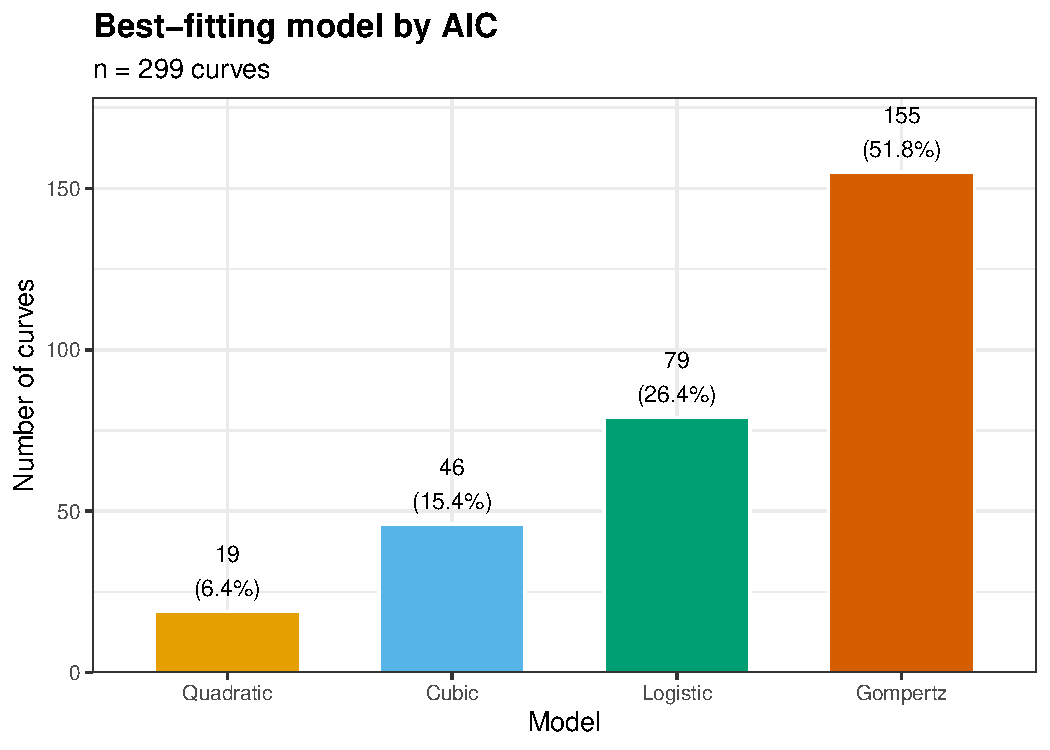
\includegraphics[width=\textwidth]{AIC_winner.pdf}
        \caption{Best-fitting models under AIC.}
        \label{fig:aic_winner}
    \end{subfigure}
    \hfill
    \begin{subfigure}[b]{0.48\textwidth}
        \centering
        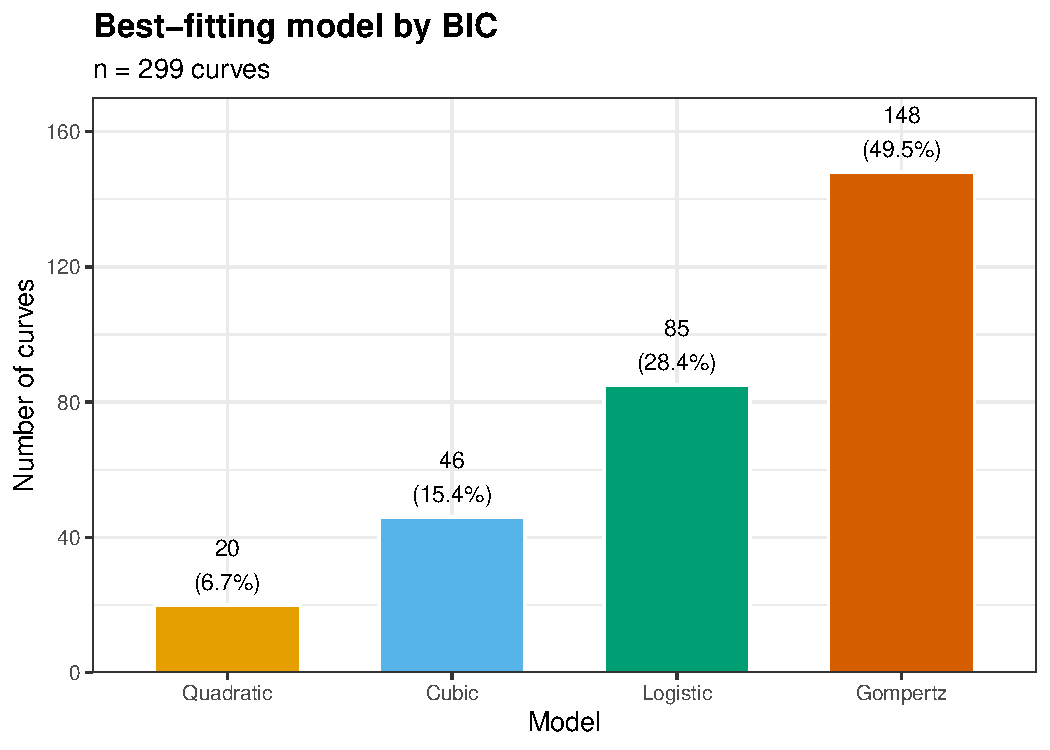
\includegraphics[width=\textwidth]{BIC_winner.pdf}
        \caption{Best-fitting models under BIC.}
        \label{fig:bic_winner}
    \end{subfigure}
    \caption{Comparison of best-fitting models selected by AIC and BIC.}
    \label{fig:aic_bic_winner}
\end{figure}
\subsection{Agreement between AIC and BIC}
AIC and BIC showed a high consistency in best-fit model selection. Within the valid 299 growth curves, around 97\% of the cases, both model selection criteria chose the same best-fit model. Interestingly, under BIC, the number of times that modified Gompertz selected as the best-fit model was slightly lower than that under AIC. This showed that some curves that were best fitted by the Gompertz model under AIC were instead assigned to the logistic growth model under BIC, since BIC applied a stricter penalty on model complexity.

\subsection{Convergence of nonlinear models}
Both nonlinear model showed a high convergence rates (Figure 2). 285 out of 299 curves converged when fitted with the logistic growth model (95.3\%), while 292 out of 299 curves converged when fitted with the Gompertz model (97.7\%). 
\begin{figure}[H]
    \centering
    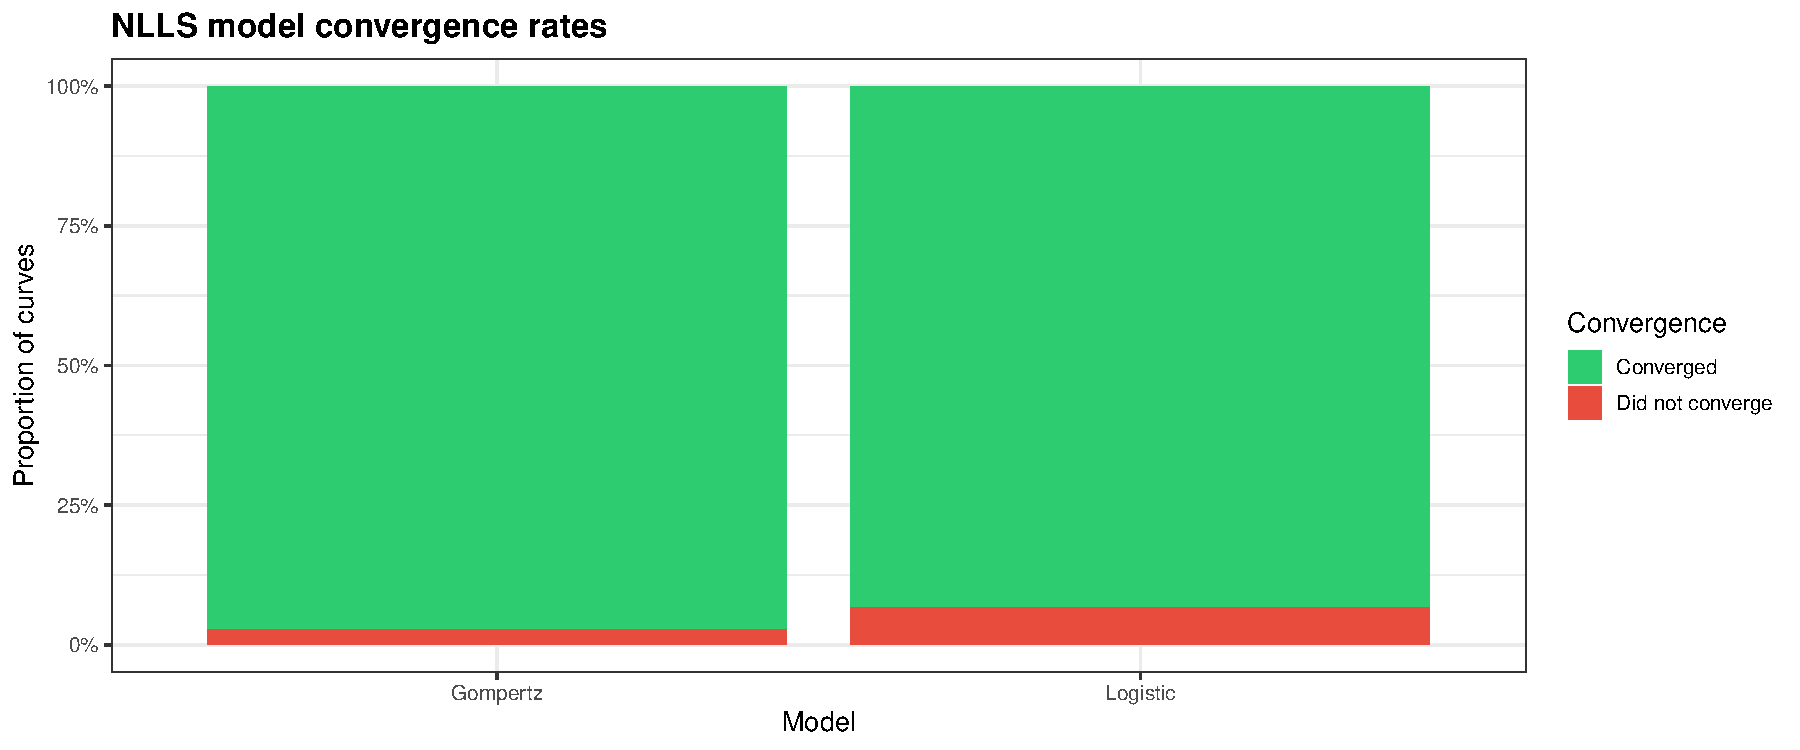
\includegraphics[width=0.75\textwidth]{convergence_rates.pdf}
    \caption{\textbf{NLLS model convergence rates for logistic and modified Gompertz models.} Proportion of growth curves successfully converged (dark) and failed to converge (light) for each nonlinear model across all 299 curves subjected to NLLS fitting.}
    \label{fig:convergence_rates}
\end{figure}
\subsection{Temperature-related variation}
Temperature-related patterns were also observed in model selection and Gompertz parameter estimates. In most temperature treatment groups, the Gompertz model was most frequently selected as the best-fitting model (Figure 3 (A)). Only in the 25 °C and 35 °C treatment groups, the logistic growth model was the most frequently selected best-fitting model. In addition, the Gompertz was tied with the cubic model at 5 °C. \(r_{\max}\) tends to be higher at moderate temperatures (Figure 3(B)). Meanwhile, \(t_{\mathrm{lag}}\) tends to be short in moderate temperature and long at colder temperatures and some high-temperature treatments. But these relationships were complex, non-monotonic and confounded by species differences.
\begin{figure}[H]
    \centering
    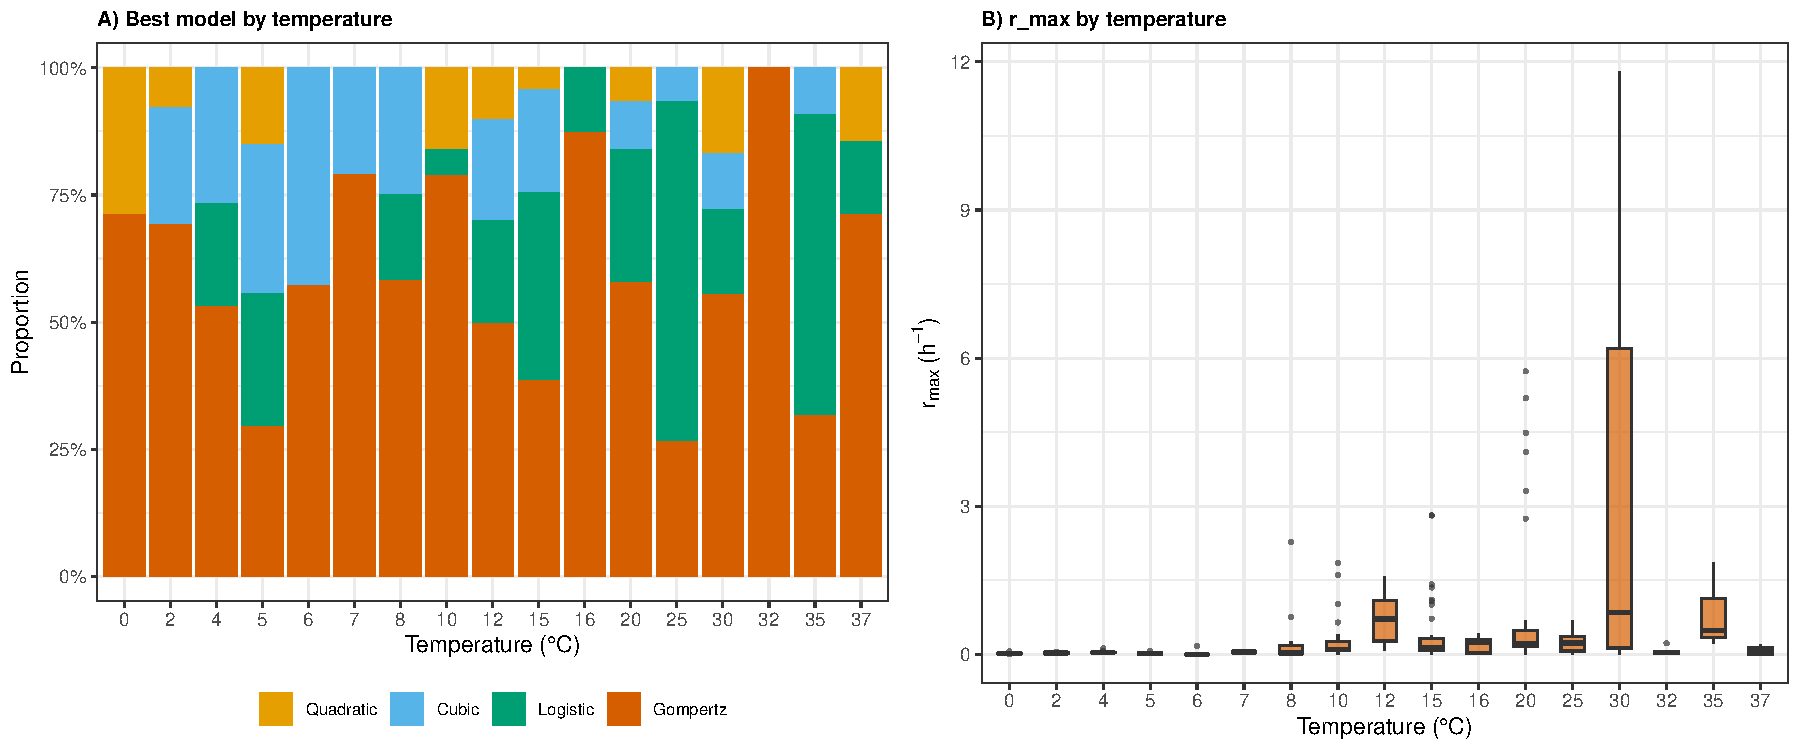
\includegraphics[width=\textwidth]{summary_temperature.pdf}
    \caption{\textbf{Model selection and maximum growth rate by temperature.}(A) Proportion of growth curves best fitted by each of the four models (quadratic, cubic, logistic, and modified Gompertz) at each temperature treatment under AIC. (B) Distribution of estimated maximum per capita growth rate rom the modified Gompertz model across temperature treatments. Each point represents a successfully converged curve. }
    \label{fig:summary_temperature}
\end{figure}
\section{Discussion}
Based on the results section, the modified Gompertz model was overall considered as the most frequently selected best-fitting model. This implied that the model can better describe and capture the microbial growth pattern (Zwietering et al., 1990). Gompertz model is one of the mechanistic models, including \(t_{\mathrm{lag}}\), a lag phase parameter, which can directly simulate the lag, exponential and stationary phases in microbial growth (Zwietering et al., 1990). This makes Gompertz model more biologically interpretable than other polynomial models (Peleg \& Corradini, 2011). In addition, this also aligns with many research findings in predictive microbiology (VANIMPE et al., 2005). In predictive microbiology, mathematical model was used to study and predict the growth pattern of microbes under different conditions, which is also a potential and important direction in food safety and storage (Baranyi \& Roberts, 1994). In this field, Gompertz model was always one of the most commonly used primary growth models. Zwietering et al. (1990)  conducted a series of experiments comparing several sigmoidal functions, suggesting that the modified Gompertz model was statistically sufficient to describe the growth curves under the tested conditions. 

Interestingly, logistic growth model was also selected as the best-fitting model when fitting some curves. This is because the logistic growth model can describe sigmoidal growth as well due to its S-shape pattern (Peleg \& Corradini, 2011). In some cases where lag phase is not present for the curves, logistic growth model itself was enough to capture the trend (Dalgaard, 1995). Also, the logistic growth model, thanks to its simpler structure and lower complexity, sometimes outperformed the modified Gompertz model under BIC, since BIC applied a stricter penalty on model complexity (Peleg \& Corradini, 2011; Schwarz, 1978; Burnham \& Anderson, 2004).

For cubic polynomial and quadratic polynomial models, they were much less frequently selected as the best-fitting model. This was due to lack of valid biological meaning of their parameters (Peleg \& Corradini, 2011). Although polynomial models can flexibly fit the shape of the curve, they can not explain the mechanism of the microbial population growth (Peleg \& Corradini, 2011). In some of the curves, they were still selected as the best-fit, which implies not all microbial growth curves perfectly match the typical sigmoidal growth trajectory (Peleg \& Corradini, 2011) . Measurement noise, incomplete coverage of the growth phases or non-typical curve shapes may help explain why polynomial models were selected as the best-fitting model for some curves (Tonner et al., 2020).

In most of the temperature treatment groups, the modified Gompertz model was still the most frequently selected as the best-fitting model. However, this leading pattern changed in 25 °C and 35 °C treatment groups, where logistic growth model became the most frequently selected best-fitting model. This suggested that, temperature-dependent variation may be present in model selection, despite the fact that these relationships were complicated and not monotonic. 

Similarly, this temperature-dependent variation also exists in the Gompertz parameter estimates. The maximum per capita growth rate \(r_{\max}\) and the lag phase period \(t_{\mathrm{lag}}\) indeed changed across different temperature treatments. As observed in the results section, \(r_{\max}\) was higher in some moderate temperatures. \(t_{\mathrm{lag}}\) tends to be longer in colder temperatures and some  high temperatures, while being shorter in some moderate temperatures. However, these relationships were not always valid and there were always outliers, which could not be simplified as a simple thermal trend. There may be several reasons for this. First of all, there were 45 species in the datasets. Each of them may have different optimal temperatures (Zwietering et al., 1990). This may lead to different lag phase periods and growth responses across different temperature treatments. Apart from this, the dataset also included different measurement types, growth media and citations, which implies that different study designs may also account for this pattern.

\section{Limitations and Link to Future Works}
First of all, the dataset contains 45 species with multiple temperature treatments, biomass measurement types, growth medium types and citation sources, which makes the dataset highly heterogeneous. Secondly, the biomass was measured with different proxies, including OD, CFU, N and dry weight. These biomass measurement proxies can not be compared directly. Finally, we only tested 4 mathematical models in this essay. Some alternative models, such as the Baranyi model or the three-phase linear model, may exhibit better fit for some curves compared to the four tested (Buchanan, Whiting \& Damert, 1997).
\section{Conclusion}
In this research, four mathematical models were tested on 299 microbial growth curves. As shown in the results, the modified Gompertz model was  most frequently selected as the best-fitting model under both AIC and BIC, with the logistic growth model ranking second. Overall, this suggested that the mechanistic models with clear and direct biological interpretability are more suitable to fit these microbial growth curves in this dataset than the two polynomial models. In the mean time, the temperature-dependent variation exists in model selection and the Gompertz model parameter estimates. However, these trends were rather complicated and may be affected by species differences and dataset heterogeneity. Alternative models and methods may enhance the overall accuracy and interpretability in the future.

\newpage
\nolinenumbers
\section{References}
\setlength{\parindent}{0pt}
\setlength{\parskip}{1.0em}
Akaike, H. (1974) A new look at the statistical model identification. \textit{IEEE Transactions on Automatic Control}. 19 (6), 716–723. doi: \url{https://doi.org/10.1109/tac.1974.1100705.}

 Auguie, B. \& Antonov, A. (2017) \textit{gridExtra: Miscellaneous Functions for ‘Grid’ Graphics}. 9 September 2017. R-Packages.{https://cran.r-project.org/web/packages/gridExtra/index.html}.

 Baranyi, J. \& Roberts, T.A. (1994) A dynamic approach to predicting bacterial growth in food. \textit{International Journal of Food Microbiology}. 23 (3-4), 277–294. doi: \url{https://doi.org/10.1016/0168-1605(94)90157-0.}

 Buchanan, R.L., Whiting, R.C. \& Damert, W.C. (1997) When is simple good enough: a comparison of the Gompertz, Baranyi, and three-phase linear models for fitting bacterial growth curves. \textit{Food Microbiology}. 14 (4), 313–326. doi: \url{https://doi.org/10.1006/fmic.1997.0125.}

 Burnham, K.P. \& Anderson, D.R. (2004) Multimodel Inference: Understanding AIC and BIC in Model Selection. \textit{Sociological Methods \& Research}. 33 (2), 261–304. doi: \url{https://doi.org/10.1177/0049124104268644.}

 Dalgaard, P. (1995) Modelling of microbial activity and prediction of shelf life for packed fresh fish. \textit{International Journal of Food Microbiology}. 26 (3), 305–317. doi: \url{https://doi.org/10.1016/0168-1605(94)00136-t.}

 Elzhov, T.V., Mullen, K.M., Spiess, A.-N. \& Bolker, B. (2023) \textit{minpack.lm: R Interface to the Levenberg-Marquardt Nonlinear Least-Squares Algorithm Found in MINPACK, Plus Support for Bounds}. 11 September 2023. R-Packages. {https://cran.r-project.org/web/packages/minpack.lm/index.html}.

 Monod, J. (1949) The Growth of Bacterial Cultures. \textit{Annual Review of Microbiology}. 3 (1), 371–394. doi: \url{https://doi.org/10.1146/annurev.mi.03.100149.002103.}

 Nielsen, J., Villadsen, J. \& Lidén, G. (2003) \textit{Bioreaction Engineering Principles}. Boston, MA, Springer US. doi: \url{https://doi.org/10.1007/978-1-4615-0767-3.}

 Peleg, M. \& Corradini, M.G. (2011) Microbial Growth Curves: What the Models Tell Us and What They Cannot. \textit{Critical Reviews in Food Science and Nutrition}. 51 (10), 917–945. 
 doi: \url{https://doi.org/10.1080/10408398.2011.570463.}

 Perez-Rodriguez, F. \& Valero, A. (2012) \textit{Predictive Microbiology in Foods}. Springer Nature. doi: \url{https://doi.org/10.1007/978-1-4614-5520-2.}

 Schwarz, G. (1978) Estimating the Dimension of a Model. \textit{The Annals of Statistics}. 6 (2), 461–464. doi: \url{https://doi.org/10.2307/2958889.}

 Tonner, P.H., Darnell, C.L., Francesca M.L. Bushell, Lund, P., Schmid, A.K. \& Schmidler, S.C. (2020) A Bayesian non-parametric mixed-effects model of microbial growth curves. \textit{PLOS COMPUTATIONAL BIOLOGY}. 16 (10), e1008366–e1008366. doi: \url{https://doi.org/10.1371/journal.pcbi.1008366.}

 VANIMPE, J., POSCHET, F., GEERAERD, A. \& VEREECKEN, K. (2005) Towards a novel class of predictive microbial growth models. \textit{International Journal of Food Microbiology}. 100 (1-3), 97–105. doi: \url{https://doi.org/10.1016/j.ijfoodmicro.2004.10.007.}

 Wickham, H. (2019) Create Elegant Data Visualisations Using the Grammar of Graphics [R package ggplot2 version 3.2.1]. \textit{R-project.org}. doi: \url{https://cran.r-project.org/package=ggplot2.}

 Wickham, H., François, R., Henry, L., Müller, K. \& RStudio (2020) \textit{dplyr: A Grammar of Data Manipulation}. 18 August 2020. R-Packages. {https://cran.r-project.org/web/packages/dplyr/index.html}.

 Wickham, H. \& Henry, L. (2020) \textit{tidyr: Tidy Messy Data}. 24 January 2020. R-Packages. {https://cran.r-project.org/web/packages/tidyr/index.html}.

 Zwietering, M.H., Jongenburger, I., Rombouts, F.M. \& van ’t Riet, K. (1990) Modeling of the Bacterial Growth Curve. \textit{Applied and Environmental Microbiology}. 56 (6), 1875–1881. doi: \url{https://doi.org/10.1128/aem.56.6.1875-1881.1990.}

 

\end{document}